\chapter{Depth-Color Fusion} \label{depthcolor}

Chapter \ref{system} presented an integrated vision system that introduces representations for images and 
camera sensors in the \RD{} development platform. In this chapter these representations are used to create
new vision-related entities. It focuses specifically on merging the representations of the color and 3D 
time-of-flight cameras with the goal of creating a new camera that provides color and depth information. 

To achieve this, it is necessary to describe an algorithm that finds correspondences between points in the 
color camera and points in the 3D camera. The first part of this chapter, Section \ref{cameras}, gives an 
overview of the setup and discusses the type of data acquired by these cameras. Then, Section \ref{algorithm} 
provides a detailed description of the depth-color fusion algorithm, using as reference the work by Linarth 
\textit{et al.} \cite{Linarth}. This algorithm consists of extracting the cameras' parameters through synchronized 
camera calibration, computing the relative transformation between both cameras, and finding the 
correspondences between color and depth pixels.

Finally, Section \ref{implementation} discusses the implementation of the fusion algorithm as part of the 
integrated vision system. This section introduces the new depth-color camera representation, as well as the
entities that are needed to perform the synchronized camera calibration and the fusion between the depth 
and color images.


\section{Cameras Setup} \label{cameras}
\begin{figure}[t]
	\center
	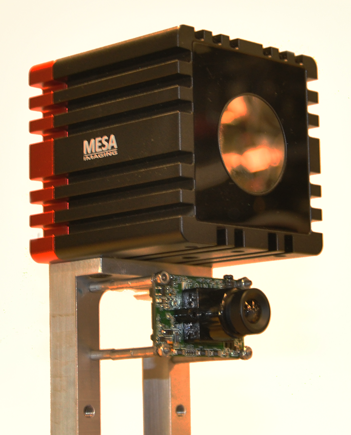
\includegraphics[width = 5cm]{camerasetup.png}
	\caption[SwissRanger depth camera and Firefly color camera setup]{SwissRanger depth 
		camera (top) and Firefly color camera (bottom) setup.}
	\label{camerassetup}
\end{figure}

Figure \ref{camerassetup} shows a setup of two camera sensors fixed on a frame, one below the other. The 
camera at the bottom is a Firefly, a Firewire camera manufactured by Point Grey \cite{FireflyDatasheet}. 
It captures grayscale images that can be converted to color using functions from the libdc1394 library
(see Section \ref{dc1394javaacquire}). The size of the images captured by a Firefly is $640 \times 480$ 
pixels.

The camera on top is a SwissRanger SR4000, a 3D time-of-flight camera manufactured by Mesa Imaging. 
It captures x-coordinate, y-coordinate, and z-coordinate information from the scene 
in front of the camera. This chapter focuses on the z-coordinate data, which will be referred to from this point 
on as the \textit{depth image}.\footnote{Similarly, the SwissRanger camera will also be referred to as the 
\textit{depth camera}.} The SwissRanger also produces an amplitude image, which corresponds to 
the amplitude of the modulated signal used in the depth measurements. The amplitude image can be used 
both for generating a grayscale image representing the captured scene and for measuring the quality of the 
depth values \cite{SR4000Manual}. The size of all images captured by the SwissRanger is $176 \times 144$
pixels.

Depending on the lens in the Firefly, the field of view of the color camera can be inside the field of view of the 
SwissRanger, or vice versa. Since the Firefly is more flexible in the matter of changing its field of view, this 
setup uses a wide angle lens on the color camera that makes it encompass the field of view of the depth 
camera. Figure \ref{imagetypes} shows an example of the three types of images captured by this 
depth-color camera setup. 
 

\begin{figure}[t]
	\center
	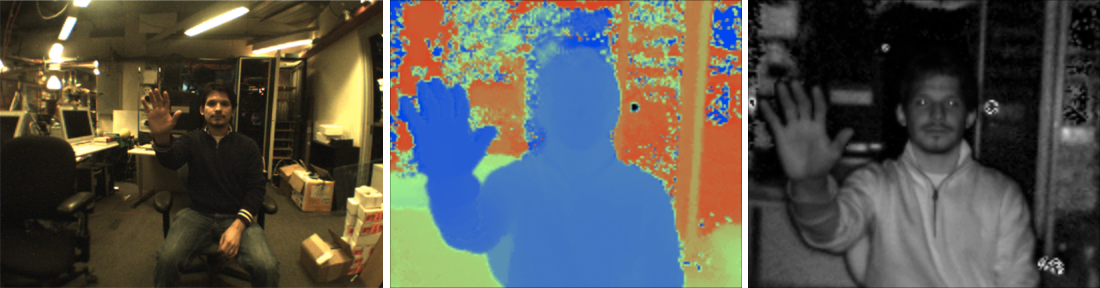
\includegraphics[width = 15cm]{data.png}
	\caption[Image types captured by the depth-color camera setup]{Image types captured by the 
		depth-color camera setup. From left to right: color image, depth image, and amplitude image.
		Notice the difference between the field of views of both cameras.}
	\label{imagetypes}
\end{figure}

\section{Fusion Algorithm} \label{algorithm}
The goal of the depth-color fusion algorithm is to find the correspondences between the pixels of a depth 
image and the pixels of a color image that have been acquired with a depth-color camera setup like the one 
described in Section \ref{cameras}. The first step of the algorithm is to retrieve the intrinsic and extrinsic 
parameters from both cameras. This is achieved by performing synchronized camera calibration. 

Given the cameras' parameters, the next step computes the relative transformation between the depth 
and color cameras, which is described in terms of a rotation and a translational offset. The relative 
transformation is used to transform world points in the depth camera's coordinate system to world points in
the color camera's coordinate system. The correspondences between points in the depth image and points 
in the color image are retrieved from an image point to world point transformation, followed by a world point 
to image point transformation.


\subsection{Cameras Calibration} \label{camerascalibration}


The depth and color cameras need to be calibrated in order to retrieve their intrinsic and extrinsic 
parameters. Since the goal is to find how the cameras are positioned and oriented one with respect to the 
other, the calibration of the cameras needs to be performed synchronously. In other words, there needs
to exist a positional correspondence between the calibration images taken with both cameras. This is 
achieved by setting the calibration pattern in a fixed position with respect to the camera setup and capturing 
one image from each camera at the same time. The two synchronized images are called an 
\textit{image pair} (see Figure \ref{imagepair}). 

\begin{figure}[t]
	\center
	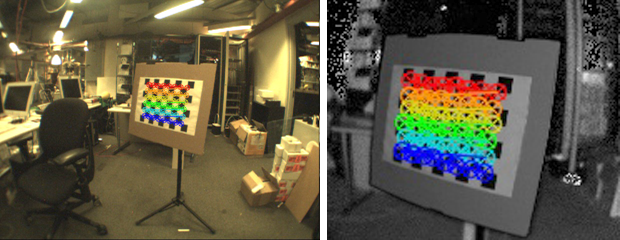
\includegraphics[width = 15cm]{imagepair.png}
	\caption[Example of a calibration image pair]{Example of a calibration image pair. An image pair is 
	composed of a color image (left) and an amplitude image from the depth camera (right).}
	\label{imagepair}
\end{figure}

As observed in Figure \ref{imagepair}, the image pair consists of a color image and an amplitude image. 
Since the amplitude image is visually similar to a grayscale image, it is possible to use it in the calibration 
process to find the calibration pattern. The colored circles in the figure indicate the location of the corners
in the pattern (see Section \ref{calibrationtool}). Besides knowing the correspondence between the images 
in an image pair, the synchronized calibration algorithm needs to know the correspondence between the 
calibration points in the two images.

The calibration process described in Section \ref{calibrationtool} computes the camera's focal length and 
principal point. If $f$ is the focal length of a camera, and $m_x$, $m_y$ are the ratios of pixel width and pixel 
height per unit distance, respectively, then $(f_x, f_y)$ represents the focal length expressed in units of 
horizontal and vertical pixels. That is, 
\begin{align}
(f_x, f_y) = ( f m_x , f m_y)
\end{align}

Furthermore, $(x_0, y_0)$ represents the principal point of the camera. Assuming that the skew coefficient 
between the $x$ and $y$ axes is zero, the intrinsic matrix of this camera is given by 
\begin{align} \label{intrinsicmatrix}
\mathbf{K} = \begin{bmatrix}
	f_x & 0    & x_0 \\
	0    & f_y & y_0 \\
	0    & 0    & 1      \\
\end{bmatrix}
\end{align}

The calibration process also provides a rotation matrix and a translation vector. These parameters describe
the transformation between the world's coordinate system and the camera's coordinate system. If 
$\mathbf{R}$ denotes the $3 \times 3$ rotation matrix, and $\mathbf{t}$ denotes the $3 \times 1$ 
translation vector, the extrinsic matrix of this camera is given by the $3 \times 4$ matrix 
\begin{align} \label{extrinsicmatrix}
\begin{bmatrix} \mathbf{R} & \mathbf{t} \\ \end{bmatrix}
\end{align}

Therefore, the synchronized calibration algorithm outputs two intrinsic matrices, $\mathbf{K}_d$ and 
$\mathbf{K}_c$, and two extrinsic matrices, $[ \mathbf{R}_d ~ \mathbf{t}_d ]$ and 
$[ \mathbf{R}_c ~ \mathbf{t}_c ]$, where the $d$ and $c$ subscripts are used to differentiate between the 
depth camera's parameters and the color camera's parameters. While the intrinsic matrices contain 
information about the internals of the camera, the extrinsic matrices hold information about how the 
cameras are positioned in space. This information is used in the next section to compute the relative 
transformation between both cameras. 


\subsection{Relative Transformation} \label{relativetransformation}


When computing the relative transformation between the cameras, the direction of the transformation is 
chosen to be from the depth camera to the color camera. As discussed in Section \ref{cameras}, the field
of view of the depth camera is within the field of view of the color camera. Therefore, every point in the depth
image will have a corresponding point in the color image, but not necessarily vice versa.

If $\mathbf{P} = (X, Y, Z)^T$ is a point in world coordinates, the position of $\mathbf{P}$ in the depth 
camera's coordinate system is given by $\mathbf{q}_d$. Similarly, the position of $\mathbf{P}$ in the color 
camera's coordinate system is given by $\mathbf{q}_c$. The points $\mathbf{q}_d$ and $\mathbf{q}_c$ 
can be expressed in terms of the cameras' extrinsic parameters by equations \eqref{qd} and \eqref{qc}, 
respectively.
\begin{align}
\mathbf{q}_d = \mathbf{R}_d \mathbf{P} + \mathbf{t}_d	\label{qd} \\
\mathbf{q}_c = \mathbf{R}_c \mathbf{P} + \mathbf{t}_c  	\label{qc}
\end{align}

Considering now the image of $\mathbf{P}$ in the depth image as having coordinates $(x_d, y_d)$, this
point can be expressed in homogeneous coordinates as $\mathbf{p}_d = (w x_d, w y_d, w )^T$, for some 
constant $w$. Using the depth camera's intrinsic parameters, $\mathbf{p}_d$ can be expressed by the 
equation:
\begin{align}
	\mathbf{p}_d = \mathbf{K}_d \mathbf{q}_d \label{pd}
\end{align}

This automatically reveals another expression for $\mathbf{q}_d$:
\begin{align}
	\mathbf{q}_d  = \mathbf{K}_{d}^{-1} \mathbf{p}_d \label{qd2}
\end{align}

Combining the two expressions for $\mathbf{q}_d$ (equations \eqref{qd} and \eqref{qd2}), and solving for 
$\mathbf{P}$ gives an equation for point $\mathbf{P}$:
\begin{align}
	\mathbf{K}_{d}^{-1} \mathbf{p}_d &= \mathbf{R}_d \mathbf{P} + \mathbf{t}_d \nonumber \\
	\mathbf{R}_d \mathbf{P} &= \mathbf{K}_{d}^{-1} \mathbf{p}_d - \mathbf{t}_d  \nonumber \\
	\mathbf{P} &= \mathbf{R}_{d}^{-1} \mathbf{K}_{d}^{-1} \mathbf{p}_d - \mathbf{R}_{d}^{-1} \mathbf{t}_d  
\end{align}

This expression for $\mathbf{P}$ can be substituted in equation \eqref{qc} to get a new expression for 
$\mathbf{q}_c$:
\begin{align}
	\mathbf{q}_c &= \mathbf{R}_c (\mathbf{R}_{d}^{-1} \mathbf{K}_{d}^{-1} \mathbf{p}_d 
					- \mathbf{R}_{d}^{-1} \mathbf{t}_d  ) + \mathbf{t}_c \nonumber \\
			    & =  \mathbf{R}_c \mathbf{R}_{d}^{-1} \mathbf{K}_{d}^{-1} \mathbf{p}_d
			    		 - \mathbf{R}_c \mathbf{R}_{d}^{-1} \mathbf{t}_d + \mathbf{t}_c \label{qc2}
\end{align}

Using equation \eqref{qd2}, equation \eqref{qc2} simplifies to:
\begin{align}
	\mathbf{q}_c &=  (\mathbf{R}_c \mathbf{R}_{d}^{-1}) ~ \mathbf{q}_{d}  
		+ (\mathbf{t}_c - \mathbf{R}_c \mathbf{R}_{d}^{-1} \mathbf{t}_d) \label{qc3}
\end{align}

Equation \eqref{qc3} reveals how the world points in the depth camera's coordinate system are related to 
the world points in the color camera's coordinate system. As seen from the equation, this
transformation is given in terms of the cameras' extrinsic parameters. Therefore, the relative transformation
between the depth and color cameras is defined by the rotation matrix in equation \eqref{relativerotation}
and the translation vector in equation \eqref{relativetranslation}.
\begin{align}
	\mathbf{R}_r = \mathbf{R}_c \mathbf{R}_{d}^{-1} \label{relativerotation} \\
	\mathbf{t}_r = \mathbf{t}_c - \mathbf{R}_r \mathbf{t}_d \label{relativetranslation}
\end{align}


\subsection{Point Correspondences} \label{pointcorrespondences}


The fusion algorithm must convert every point $(x_d, y_d)$ in the depth image into a point $(x_c, y_c)$ in 
the color image. This is achieved by first computing the world point $\mathbf{q}_d$ from the depth image
point $(x_d, y_d)$. Then, $\mathbf{q}_d$ is transformed into $\mathbf{q}_c$ using the results from Section 
\ref{relativetransformation}. Finally, world point $\mathbf{q}_c$ is converted into a color image point 
$(x_c, y_c)$.

If $(f_x, f_y)$ and $(x_0, y_0)$ are the focal length and principal point of the depth camera, respectively, 
the world point $\mathbf{q}_d = (X, Y, Z)^T$ can be related to the image point $(x_d, y_d)$ through the 
perspective projection equations \eqref{xd} and \eqref{yd}. 
\begin{align}
	x_d &= f_x \frac{X}{Z} + x_0 \label{xd} \\
	y_d &= f_y \frac{Y}{Z} + y_0 \label{yd} 
\end{align}
	
The depth camera provides the $z$-component of $\mathbf{q}_d$.\footnote{The depth camera can actually 
provide all components as discussed in Section \ref{cameras}. However, the noise in these measurements is 
high and recomputing the $x$ and $y$ components delivers better results.}
The $x$ and $y$ components are computed by solving equations \eqref{xd} and \eqref{yd} for $X$ and 
$Y$, respectively:
\begin{align}
	X = \frac{Z}{f_x} (x_d - x_0) \label{X} \\
	Y = \frac{Z}{f_y} (y_d - y_0) \label{Y}
\end{align}

Using the color camera's intrinsic parameters, $\mathbf{p}_c$ can be expressed by the equation
\begin{align}
	\mathbf{p}_c = \mathbf{K}_c \mathbf{q}_c \label{pc}
\end{align}

Furthermore, equation \eqref{qc3} gives an expression for $\mathbf{q}_c$. Therefore, combining 
\eqref{pc} and \eqref{qc3} results in a new equation for $\mathbf{p}_c$:
\begin{align}
	\mathbf{p}_c &=  \mathbf{K}_c (\mathbf{R}_r \mathbf{q}_{d}  + \mathbf{t}_r) \label{pc2}
\end{align}

By expressing $\mathbf{q}_{d}$ in homogeneous coordinates (that is, $\mathbf{q}_{d}^{'} = (X, Y, Z, 1)^T$), 
equation \eqref{pc2} can be rewritten as 
\begin{align}
	\mathbf{p}_c &=  \mathbf{K}_c [\mathbf{R}_r  ~  \mathbf{t}_r] \mathbf{q}_{d}^{'} \label{pc3}
\end{align}

The image coordinates $(x_c, y_c)$ are obtained by dividing the first and second components of 
$\mathbf{p}_c$ by its third component. That is, if $\mathbf{p}_c = (x,y,z)^T$, then 
\begin{align}
	(x_c, y_c) = \Bigg( \frac{x}{z} , \frac{y}{z} \Bigg) \label{xcyc}
\end{align}




\section{Implementation in the Vision System} \label{implementation}
	
The vision system described in Chapter \ref{system} provides the core structure needed to implement the 
depth-color fusion algorithm. The implementation is introduced in the form of a new camera object that 
provides fused depth-color images. The following sections discuss the classes that make up this 
representation, and the module dependency diagram in Figure \ref{depthcolorcammoduledependency} 
illustrates how they are related to the components of the vision system.

\begin{figure}[t]
\begin{center}
\digraph[scale=0.72]{DepthColorCam}{
	graph [rankdir = "TB" margin = 0];
	node [shape = "box" style = "filled" fillcolor = "gainsboro" fontsize = "12" fontname = "Courier"];
		Camera CameraData;
	node [shape = "box" style = "filled" fillcolor = "floralwhite" fontsize = "12" fontname = "Courier"];
	{ rank = "source"; Camera CameraData;}
	{ rank = "same"; DepthColorCam DepthColorCamData;}
	{ rank = "same"; ColorCam SwissRangerCam;}
	{ rank = "same"; DepthColorCalibrationTool DepthColorFusion;}
	{ rank = "sink"; CalibrationTool ;}
	edge [arrowhead = "normal"];
	Camera -> CameraData;
	DepthColorCam -> Camera [arrowhead = "empty"] ;
	DepthColorCam -> DepthColorCamData;
	DepthColorCam -> DepthColorCalibrationTool;
	DepthColorCam -> DepthColorFusion;
	DepthColorCam -> ColorCam;
	DepthColorCam -> SwissRangerCam;
	DepthColorCamData -> CameraData [arrowhead = "empty"];
	DepthColorCalibrationTool -> CalibrationTool;
	ColorCam -> CalibrationTool;
	SwissRangerCam -> CalibrationTool;
}
\caption[\DepthColorCam{}'s module dependency diagram]{\DepthColorCam{} module dependency diagram. 
Arcs with white arrows represent subtype relations (A $\vartriangleright$ B = A extends B) while arcs with 
black arrows represent implementation relations (A $\blacktriangleright$ B = A uses B). Gray rectangles 
represent abstract classes. The \ImageBuffer{} class is omitted from this diagram.}
\label{depthcolorcammoduledependency}
\end{center}
\end{figure}

	\subsection{Depth-Color Camera} \label{depthcolorcam}
	The \DepthColorCam{} class represents a camera that provides fused depth-color images. It extends the 
\Camera{} abstract class, the base camera representation discussed in Section \ref{camera}. The 
implementation of the \DepthColorCam{} class, however, differs from that of the \ColorCam{} and 
\SwissRangerCam{} classes (see Sections \ref{colorcam} and \ref{swissrangercam}). The principal reason for 
the difference comes from the fact that instead of representing an actual sensor device, this class represents 
the merging of a depth camera with a color camera through the algorithmic process discussed in Section 
\ref{algorithm}.

In order to respond to this representation, the \DepthColorCam{} class instantiates a \SwissRangerCam{} 
object and a \ColorCam{} object. As discussed before, this means the acquired depth and color images can
either come directly from the cameras or be transferred through the network. Before obtaining the fused 
images, the depth-color camera needs to be calibrated using the \DepthColorCalibrationTool{}. This 
calibration tool provides the cameras' parameters needed by the \DepthColorFusion{} class to fuse the 
acquired depth and color images.

Table \ref{depthcolorcammethods} lists the methods of the \DepthColorCam{} class. The depth-color camera
object provides access to the fused image through the \texttt{get\-Fused\-Col\-or} and \texttt{get\-Depth}
methods. The first method returns the image buffer containing the color information of the fused image. The
second method returns the image buffer containing the depth information. The camera object also provides
access to the original color image (\texttt{get\-O\-rig\-i\-nal\-Col\-or}) and to the amplitude image associated 
with the depth measurements (\texttt{get\-Am\-pli\-tude}).

\begin{table}[ht]
\caption{Public methods in the \DepthColorCam{} class}
\begin{center}
\begin{tabular}{| l |}
	\hline 
	\multicolumn{1}{| c |}{\DepthColorCam{}} \\
	\multicolumn{1}{| c |}{{\small \texttt{extends} \Camera{}}} \\
	\hline \hline
	\texttt{getFusedColor} \\
	\texttt{getDepth} \\
	\texttt{getAmplitude} \\
	\texttt{getOriginalColor} \\
	\texttt{getDepthDisplay} \\
	\texttt{getAmplitudeDisplay} \\
	\texttt{getFusedColorView} \\
	\texttt{getDepthView} \\
	\texttt{getAmplitudeView} \\
	\texttt{getOriginalColorView} \\
	\texttt{getFusionTool} \\
	\texttt{getCalibrationTool} \\
	\texttt{getModulationFrequency} \\
	\texttt{setCameraParameters} \\
	\texttt{setupDepthColorFusion} \\
	\hline
\end{tabular}
\end{center}
\label{depthcolorcammethods}
\end{table}

Like the \SwissRangerCam{} class, the depth-color camera provides image buffers with the color
visualizations of the depth and amplitude images. These visualizations are obtained through the 
\texttt{get\-Depth\-Dis\-play} and \texttt{get\-Am\-pli\-tude\-Dis\-play} methods. Furthermore, all image streams
(fused color, depth, amplitude, and original color) are displayed in \RD{} using the \ImageView{} objects that 
are associated with each image buffer.

The rest of the methods are used to retrieve the modulation frequency on which the SwissRanger camera is
operating, to gain access to the \DepthColorCalibrationTool{} and \DepthColorFusion{} objects associated
with the depth-color camera, and to setup the depth-color fusion object after the camera has been calibrated. 

When capturing the image stream from the depth and color cameras, it is important to make sure that the
pair of acquired images belongs to the same point in time. Since the camera devices are different, the time
response of their capturing mechanisms is not identical. Furthermore, the transfer of the images from the 
cameras to the computer running \RD{} also accounts for the time difference between the 
images.\footnote{For example, the computer's processor speed might affect the image transfer time.}

To solve this synchronization problem, the depth-color camera uses the version of the \texttt{grab\-Im\-age} 
method in the \ColorCam{} and \SwissRangerCam{} objects that takes as input the desired timestamp of the 
image that will be grabbed (see Sections \ref{colorcam} and \ref{swissrangercam}). By using this method it is
possible to retrieve the two images closest in time while taking into account the timestamp offset. Table 
\ref{depthcolorgrabimage} describes the algorithm used by the \texttt{grab\-Im\-age} method in the 
depth-color camera to retrieve the depth and color images and produce the fused image.

\begin{table}[ht]
\caption[Algorithm for the \texttt{grabImage} method in \DepthColorCam{}]{Algorithm for the 
\texttt{grabImage} method in \DepthColorCam{}. The method returns \texttt{true} if the image  
was grabbed successfully and \texttt{false} otherwise.}
\begin{center}
\begin{tabular}{ l l }
\hline
\multicolumn{2}{l}{\texttt{GRAB\_IMAGE :}} \\
1 & \texttt{Grab image from color camera;} \\
2 & \texttt{{\bf If} the image is grabbed successfully} \\
3 & \hspace{0.6cm} \texttt{\bf Then:} \\
4 & \hspace{1.2cm} \texttt{Grab image from SwissRanger camera using as} \\
-  & \hspace{1.8cm} \texttt{input the timestamp of the color image;} \\
5 & \hspace{1.2cm} \texttt{{\bf If} the image is grabbed successfully} \\
6 & \hspace{1.8cm} \texttt{\bf Then:} \\
7 & \hspace{2.4cm} \texttt{Fuse the color and depth images;} \\
8 & \hspace{2.4cm} \texttt{Return true;} \\
9 & \hspace{1.8cm} \texttt{\bf Else:} \\
10 & \hspace{2.4cm} \texttt{Return false;} \\
11 & \hspace{0.6cm}\texttt{\bf Else:} \\
12 & \hspace{1.2cm} \texttt{Return false;} \\
\hline
\end{tabular}
\end{center}
\label{depthcolorgrabimage}
\end{table}

Another problem that arises with the depth-color camera involves the noisy nature of the SwissRanger
images. As mentioned in Section \ref{pointcorrespondences}, the noisy values for the $x$ and $y$ 
coordinates provided by the SwissRanger camera are discarded and recalculated using equations \eqref{X} 
and \eqref{Y}. The depth values, however, cannot be recalculated. The noise from the depth data produces 
a fused color image like the one shown in Figure \ref{noise}. In order to reduce this noise, some depth 
values are discarded based on depth and amplitude thresholds. Points that are too close, points that are too 
far, and points with small amplitude value are discarded. This produces areas with no depth and color 
information in the final fused depth-color image. 

\begin{figure}[t]
\center
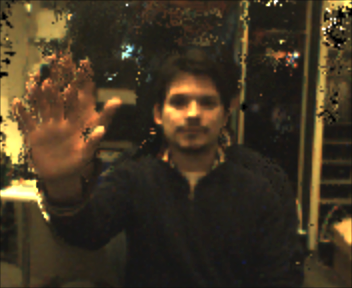
\includegraphics[scale = 0.5]{fusedcolornoise.png}
\caption{Fused color image without noise reduction}
\label{noise}
\end{figure}

Figure \ref{fusion} illustrates the result provided by the depth-color camera. It shows the original depth 
and color images, and next to them the fused color image. The black pixels in the depth and fused color
images indicate the points that were discarded due to data noise. It is worth noting that by thresholding the 
depth image it is possible to segment the object of interest from the background. 

\begin{figure}[t]
\center
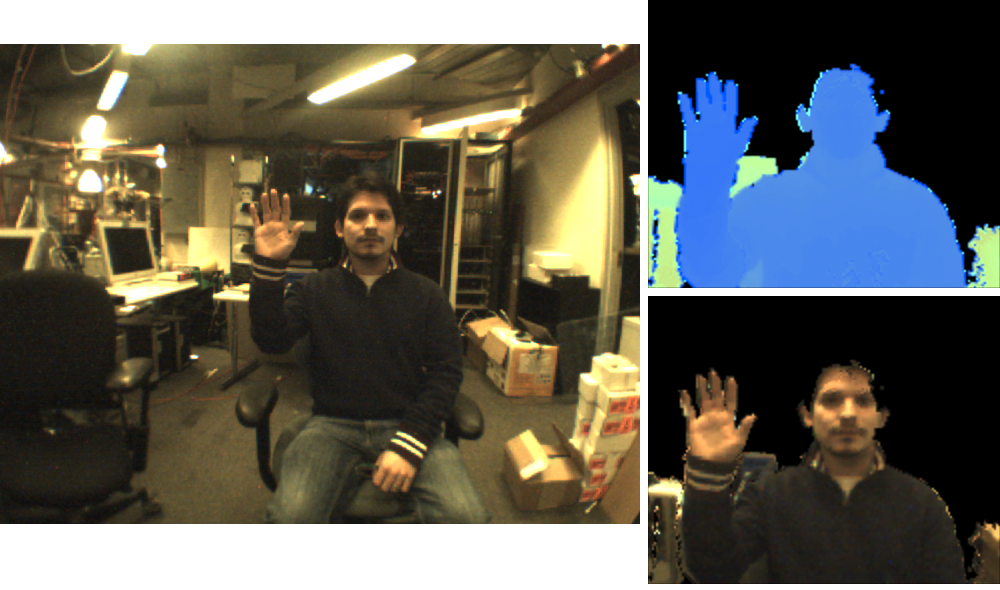
\includegraphics[width = 15cm]{fusion.png}
\caption[\DepthColorCam{}'s images]{\DepthColorCam{}'s images: the original color image (left), the 
depth image (upper right) and the fused color image (bottom right).}
\label{fusion}
\end{figure}



	
	\subsection{Depth-Color Calibration Tool} \label{depthcolorcalibrationtool}
	The \DepthColorCalibrationTool{} class implements the steps of the depth-color fusion algorithm that are 
described in Sections \ref{camerascalibration} and \ref{relativetransformation}. Analogous to the 
\DepthColorCam{} class, the implementation uses two \CalibrationTool{} objects, one for each of the cameras 
that is to be calibrated. The idea behind it consists of performing the calibration of both cameras in parallel, 
accepting an image pair only when the calibration pattern is found in both images.

Table \ref{depthcolorcalibrationtoolmethods} lists the methods of the \DepthColorCalibrationTool{} class. Similar
to a \CalibrationTool{} object, a depth-color calibration tool has methods to start, reset, and retrieve the status 
of the calibration process. It also provides methods to load and save the cameras' parameters, and to change
the default values of some of the parameters in the calibration process. 

\begin{table}[ht]
\caption{Public methods in the \DepthColorCalibrationTool{} class}
\begin{center}
\begin{tabular}{| l |}
	\hline 
	\multicolumn{1}{| c |}{\DepthColorCalibrationTool{}} \\
	\hline \hline
	\texttt{start} \\
	\texttt{reset} \\
	\texttt{isCalibrating} \\
	\texttt{calibrate} \\
	\texttt{setColorCameraParameters} \\
	\texttt{setDepthCameraParameters} \\
	\texttt{setChessboardSquareSize} \\
	\texttt{setChessboardDimensions} \\
	\texttt{setRequiredSamples} \\
	\texttt{getColorCameraParameters} \\
	\texttt{getDepthCameraParameters} \\
	\texttt{getChessboardNumberOfColumns} \\
	\texttt{getChessboardNumberOfRows} \\
	\texttt{getChessboardSquareSize} \\
	\texttt{getRequiredSamples} \\
	\texttt{getRelativeRotation} \\
	\texttt{getRelativeTranslation} \\
	\texttt{getRelativeTransformation} \\
	\texttt{loadCameraParameters} \\
	\texttt{saveCameraParameters} \\ 
	\hline
\end{tabular}
\end{center}
\label{depthcolorcalibrationtoolmethods}
\end{table}

The algorithm for the \texttt{cal\-i\-brate} method in the \DepthColorCalibrationTool{} class is also similar to the 
one seen in Section \ref{calibrationtool}. However, in this case it handles two calibration processes in parallel.
Throughout the steps of the algorithm described in Table \ref{depthcolorcalibratealgorithm}, the methods
\texttt{find\-And\-Draw\-Cor\-ners}, \texttt{add\-Cor\-ners\-To\-List}, and \texttt{cal\-i\-brate\-Cam\-er\-a}  
are called simultaneously on the two calibration tool objects used by the depth-color calibration tool.

\begin{table}[ht]
\caption{Algorithm for the \texttt{calibrate} method in \DepthColorCalibrationTool{}}
\begin{center}
\begin{tabular}{ l l }
\hline
\multicolumn{2}{l}{\texttt{CALIBRATE (currentImages, requiredImages):}} \\
1 & \texttt{{\bf If} (currentImages < requiredImages)} \\
2 & \hspace{0.6cm} \texttt{\bf Then:} \\
3 & \hspace{1.2cm} \texttt{Search checkerboard pattern in color image;} \\
4 & \hspace{1.2cm} \texttt{Search checkerboard pattern in amplitude image;} \\
5 & \hspace{1.2cm} \texttt{{\bf If} the pattern is found in both images} \\
6 & \hspace{1.8cm} \texttt{\bf Then:} \\
7 & \hspace{2.4cm} \texttt{Extract corners from color image and save them;} \\
8 & \hspace{2.4cm} \texttt{Extract corners from amplitude image and save them;} \\
9 & \hspace{2.4cm} \texttt{Increment currentImages counter;} \\
10 & \hspace{0.6cm} \texttt{\bf Else:} \\
11 & \hspace{1.2cm} \texttt{Run color camera calibration with saved corners;} \\
12 & \hspace{1.2cm} \texttt{Run depth camera calibration with saved corners;} \\
13 & \hspace{1.2cm} \texttt{Compute relative transformation with computed parameters;} \\
\hline
\end{tabular}
\end{center}
\label{depthcolorcalibratealgorithm}
\end{table}

This synchronized calibration takes advantage of the underlying OpenCV calibration functions. As mentioned in 
Section \ref{calibrationtool}, the calibration is performed using the functions in the OpenCV open source library. 
The function \texttt{cv\-Find\-Chess\-board\-Cor\-ners}, for example, locates the corners of a checkerboard 
(chessboard) pattern in an image \cite{Bradski}. Since it returns the corners ordered in row-major order 
starting from the upper-left corner, it is easy to know the correspondence between the calibration points 
in the depth image and the calibration points in the color image. 

As seen in Table \ref{depthcolorcalibratealgorithm}, the success of the calibration loop depends on finding the 
calibration pattern in both images of the image pair. When the calibration is completed for both
cameras, the relative transformation is calculated using equations \eqref{relativerotation} and 
\eqref{relativetranslation}. The parameters of the transformation can be accessed through three different 
methods. The \texttt{get\-Rel\-a\-tive\-Ro\-ta\-tion} and \texttt{get\-Rel\-a\-tive\-Trans\-la\-tion} methods return 
the $3 \times 3$ rotation matrix and $3 \times 1$ translation vector, respectively. The 
\texttt{get\-Rel\-a\-tive\-Trans\-for\-ma\-tion} method returns a $3 \times 4$ matrix in the form of an extrinsic 
matrix as described by equation \eqref{extrinsicmatrix}. Both the combination of the first two methods and the 
third method by itself provide all the necessary information to describe the transformation in 3D space between 
the depth camera and the color camera.

	
	\subsection{Depth-Color Fusion} \label{depthcolorfusion}
	The \DepthColorFusion{} class implements the steps of the depth-color fusion algorithm described in Section 
\ref{pointcorrespondences}. The constructor of this class takes as input the cameras' parameters 
computed with the \DepthColorCalibrationTool{} object. From these parameters it can calculate the relative 
transformation between the depth and color cameras using equations \eqref{relativerotation} and 
\eqref{relativetranslation}. Then, method \texttt{fuse\-Points}, listed in Table \ref{depthcolorfusionmethods},
can be used to get the point correspondences between the depth and color images.

\begin{table}[ht]
\caption{Public methods in the \DepthColorFusion{} class}
\begin{center}
\begin{tabular}{| l |}
	\hline 
	\multicolumn{1}{| c |}{\DepthColorFusion{}} \\
	\hline \hline
	\texttt{fusePoints} \\
	\texttt{getDepthCameraParameters} \\
	\texttt{getColorCameraParameters} \\
	\texttt{getDepthToColorMap} \\
	\texttt{getColorToDepthMap} \\
	\hline
\end{tabular}
\end{center}
\label{depthcolorfusionmethods}
\end{table}

Table \ref{fusepointsalgorithm} describes the algorithm for the \texttt{fuse\-Points} method. The method takes 
as input the depth image, the color image, and the image buffer where it will store the fused color information. 
For each pixel in the depth image it finds the correspondent pixel in the color image. Then, the algorithm 
retrieves the color value from the pixel in the color image and stores it in the pixel of the fused color buffer with 
position equal to the position of the depth image pixel. This fusion operation can be performed in real time with
live image streams.

\begin{table}[ht]
\caption{Algorithm for the \texttt{fusePoints} method in \DepthColorFusion{}}
\begin{center}
\begin{tabular}{ l l }
\hline
\multicolumn{2}{l}{\texttt{FUSE\_POINTS (depthImage, colorImage, fusedImage):}} \\
1 & \texttt{{\bf For} each pixel $(x_d, y_d)$ of depthImage:} \\
2 & \hspace{0.6cm} \texttt{Compute the world point $q_d$ using the depth value} \\
- & \hspace{1.2cm} \texttt{and equations \eqref{X} and \eqref{Y};} \\
3 & \hspace{0.6cm} \texttt{Compute homogeneous image point $p_c$ using equation \eqref{pc3};} \\
4 & \hspace{0.6cm} \texttt{Compute color image coordinate $(x_c, y_c)$ using equation \eqref{xcyc};} \\
5 & \hspace{0.6cm} \texttt{Retrieve color value from pixel $(x_c, y_c)$ of colorImage;} \\
6 & \hspace{0.6cm} \texttt{Place retrieved color value in pixel $(x_d, y_d)$ of fusedImage;} \\
\hline
\end{tabular}
\end{center}
\label{fusepointsalgorithm}
\end{table}

The final output of the depth-color fusion algorithm is a fused image that is composed of the original depth 
image and the fused color image. There is a one-to-one correspondence between the pixels of these images
with same $x$ and $y$ position. Furthermore, the \DepthColorFusion{} object stores the point correspondence
information in the form of two hash maps, one that maps points in the depth image to points in the original color
image, and another one that maps points in the original color image to points in the depth image. These hash
maps can be accessed through the \texttt{get\-Depth\-To\-Col\-or\-Map} and 
\texttt{get\-Col\-or\-To\-Depth\-Map} methods, respectively.





